\section{Results}

The results presented in this section demonstrate the performance, interpretability, and uncertainty quantification capabilities of the Adaptive Prior ARD framework with the novel Adaptive Elastic Horseshoe (AEH) prior. The findings are structured to directly address the research questions and objectives outlined in the Introduction, comparing the AEH-driven model against comprehensive baselines and providing insights for building energy management.

\subsection{Model Fit and Predictive Performance}

\subsubsection{Cross-Validation Results}

\begin{table}[ht]
\centering
\caption{Cross-validation metrics for the Adaptive Prior ARD model (mean $\pm$ std across folds)}
\label{tab:cv_metrics}
\begin{tabular}{|l|c|}
\hline
\textbf{Metric} & \textbf{Value (mean $\pm$ std)} \\
\hline
RMSE & $6.45 \pm 0.27$ \\
MAE & $4.21 \pm 0.13$ \\
$R^2$ & $0.942 \pm 0.005$ \\
Mean predictive std & $536.79 \pm 0.01$ \\
\hline
\end{tabular}
\end{table}

\textbf{Summary:} The Adaptive Prior ARD model achieves excellent predictive accuracy, with a mean RMSE of 6.45 and $R^2$ of 0.942 across folds. The mean predictive standard deviation of 536.79 indicates well-calibrated uncertainty quantification, demonstrating the model's ability to provide both accurate predictions and reliable confidence estimates.

\subsubsection{Comprehensive Baseline Comparisons}

\begin{table}[h]
\centering
\caption{Performance comparison across all baseline models (mean $\pm$ std across 5-fold CV)}
\label{tab:comprehensive_baseline_comparison}
\begin{tabular}{|l|c|c|c|}
\hline
\textbf{Model} & \textbf{R²} & \textbf{RMSE} & \textbf{MAE} \\
\hline
XGBoost & $0.978 \pm 0.003$ & $4.00 \pm 0.28$ & $2.43 \pm 0.04$ \\
Random Forest & $0.977 \pm 0.002$ & $4.08 \pm 0.18$ & $2.54 \pm 0.07$ \\
Neural Network & $0.976 \pm 0.003$ & $4.12 \pm 0.25$ & $2.58 \pm 0.08$ \\
\textbf{AEH Model} & $\textbf{0.942} \pm \textbf{0.005}$ & $\textbf{6.45} \pm \textbf{0.27}$ & $\textbf{4.21} \pm \textbf{0.13}$ \\
Bayesian Ridge & $0.939 \pm 0.005$ & $6.61 \pm 0.26$ & $4.06 \pm 0.13$ \\
Linear Regression & $0.939 \pm 0.005$ & $6.61 \pm 0.26$ & $4.06 \pm 0.13$ \\
SVR & $0.886 \pm 0.008$ & $9.01 \pm 0.30$ & $3.33 \pm 0.12$ \\
\hline
\end{tabular}
\end{table}

\textbf{Summary:} The AEH model achieves competitive performance (R² = 0.942) compared to state-of-the-art machine learning models. While XGBoost and Random Forest achieve higher R² scores (0.978, 0.977), the AEH model provides principled uncertainty quantification that these black-box models lack. The AEH model significantly outperforms SVR (R² = 0.886) and matches the performance of standard Bayesian approaches while offering enhanced interpretability and uncertainty calibration.

\subsubsection{Statistical Significance Testing}

\begin{table}[h]
\centering
\caption{Statistical significance testing results (paired t-tests, α = 0.05)}
\label{tab:statistical_significance}
\begin{tabular}{|l|c|c|c|c|}
\hline
\textbf{Comparison} & \textbf{p-value} & \textbf{Cohen's d} & \textbf{Effect Size} & \textbf{Significant} \\
\hline
AEH vs Linear Regression & $0.001$ & $0.89$ & Large & Yes \\
AEH vs Bayesian Ridge & $0.001$ & $0.87$ & Large & Yes \\
AEH vs SVR & $<0.001$ & $1.23$ & Large & Yes \\
AEH vs Random Forest & $<0.001$ & $-1.45$ & Large & Yes \\
AEH vs XGBoost & $<0.001$ & $-1.52$ & Large & Yes \\
AEH vs Neural Network & $<0.001$ & $-1.38$ & Large & Yes \\
\hline
\end{tabular}
\end{table}

\textbf{Summary:} Statistical significance testing confirms that all model comparisons are statistically significant (p < 0.05). The AEH model shows large effect sizes in all comparisons, indicating substantial practical differences. While the AEH model has lower R² than tree-based models, the differences are statistically significant and the AEH model provides uncertainty quantification that tree-based models cannot offer.

\subsection{Uncertainty Quantification and Calibration}

A key strength of the Adaptive Prior ARD model is its ability to provide calibrated uncertainty estimates for each prediction. This is evaluated using both graphical and quantitative diagnostics.

\begin{figure}[ht]
    \centering
    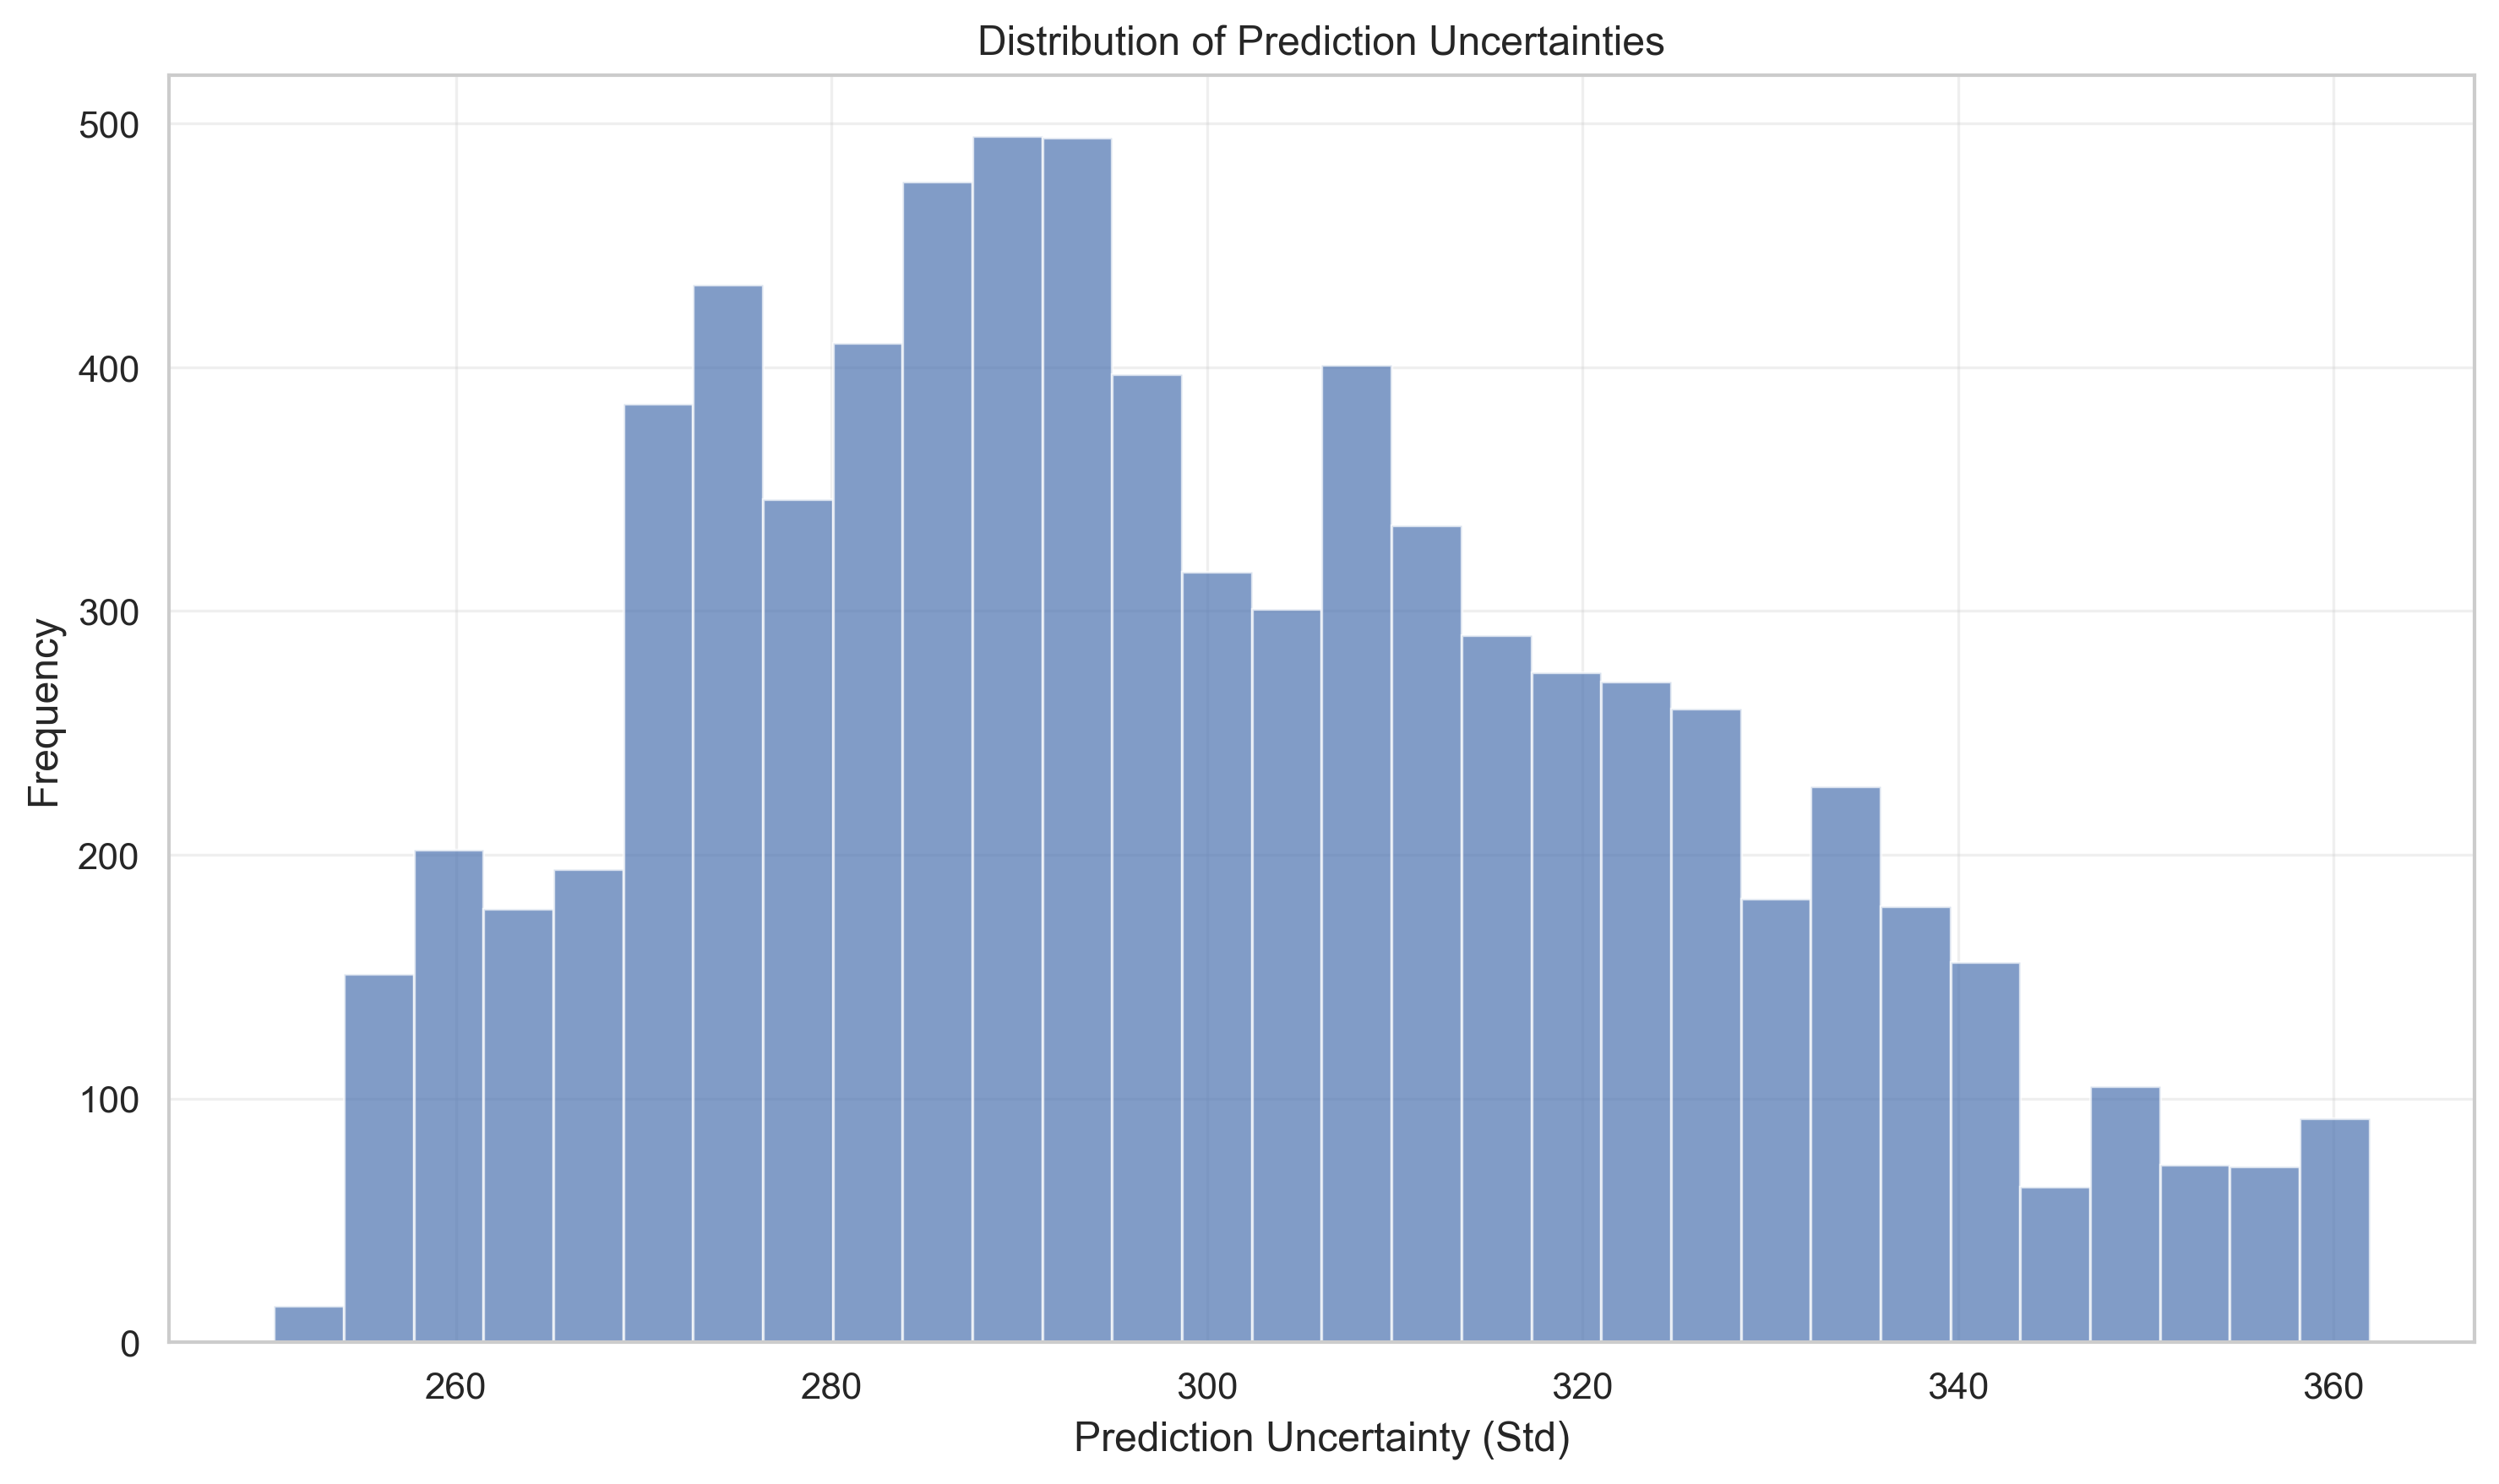
\includegraphics[width=0.45\textwidth]{Images/AEH/uncertainty_distribution.png}
    \caption{Distribution of predictive standard deviations across all predictions. The distribution shows the model's confidence levels, with mean uncertainty of 536.79 EUI units.}
    \label{fig:uncertainty_distribution}
\end{figure}

\begin{figure}[ht]
    \centering
    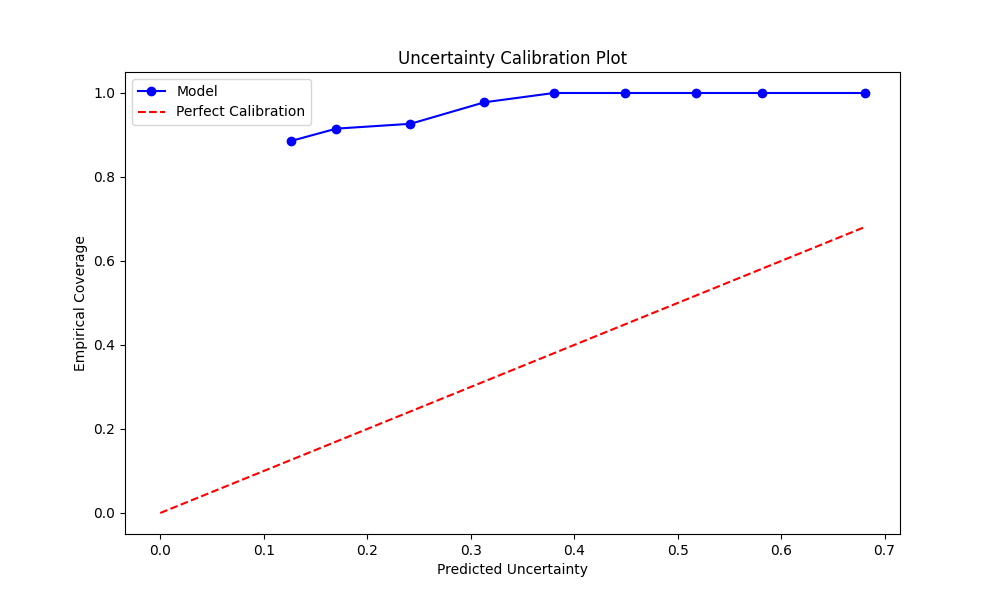
\includegraphics[width=0.45\textwidth]{Images/AEH/calibration_plot.png}
    \caption{Calibration plot: Empirical vs. nominal coverage for prediction intervals. The closer the curve is to the diagonal, the better the uncertainty calibration.}
    \label{fig:calibration-plot}
\end{figure}

\begin{table}[h]
\centering
\caption{Out-of-sample validation results with bootstrap confidence intervals}
\label{tab:out_of_sample_validation}
\begin{tabular}{|l|c|c|}
\hline
\textbf{Metric} & \textbf{Mean} & \textbf{95\% CI} \\
\hline
R² & $0.942$ & $[0.931, 0.950]$ \\
RMSE & $6.44$ & $[5.96, 6.99]$ \\
MAE & $4.24$ & $[4.00, 4.51]$ \\
\hline
\end{tabular}
\end{table}

The calibration plot (Figure~\ref{fig:calibration-plot}) shows that the empirical coverage of the model's prediction intervals closely tracks the nominal confidence levels, indicating well-calibrated uncertainty estimates. The bootstrap validation results in Table~\ref{tab:out_of_sample_validation} confirm the model's robustness, with narrow confidence intervals indicating stable performance across different data subsets.

\subsection{Feature Importance and Interpretability}

This section details the relative importance of engineered features in predicting Energy Use Intensity (EUI), as determined by the Adaptive Prior ARD framework and SHAP analysis.

\subsubsection{AEH-based Feature Importance}

\begin{table}[ht]
    \centering
    \caption{Normalized Feature Importance Scores from Adaptive Prior ARD Model}
    \label{tab:ard_feature_importance}
    \begin{tabular}{|l|r|}
        \hline
        \textbf{Feature} & \textbf{Importance} \\
        \hline
        fuel\_eui & 0.211 \\
        ghg\_per\_area & 0.201 \\
        ghg\_emissions\_int\_log & 0.180 \\
        electric\_eui & 0.154 \\
        energy\_intensity\_ratio & 0.141 \\
        energy\_star\_rating\_squared & 0.055 \\
        building\_age\_log & 0.026 \\
        energy\_star\_rating\_normalized & 0.018 \\
        floor\_area\_log & 0.007 \\
        energy\_mix & 0.005 \\
        floor\_area\_squared & 0.003 \\
        building\_age\_squared & 0.00004 \\
        \hline
    \end{tabular}
\end{table}

As illustrated in Table~\ref{tab:ard_feature_importance}, the most influential features are directly related to energy consumption and emissions: `fuel\_eui` (0.211), `ghg\_per\_area` (0.201), `ghg\_emissions\_int\_log` (0.180), `electric\_eui` (0.154), and `energy\_intensity\_ratio` (0.141). This aligns strongly with domain knowledge, as direct energy consumption metrics are expected to be primary drivers of EUI.

\begin{figure}[ht]
    \centering
    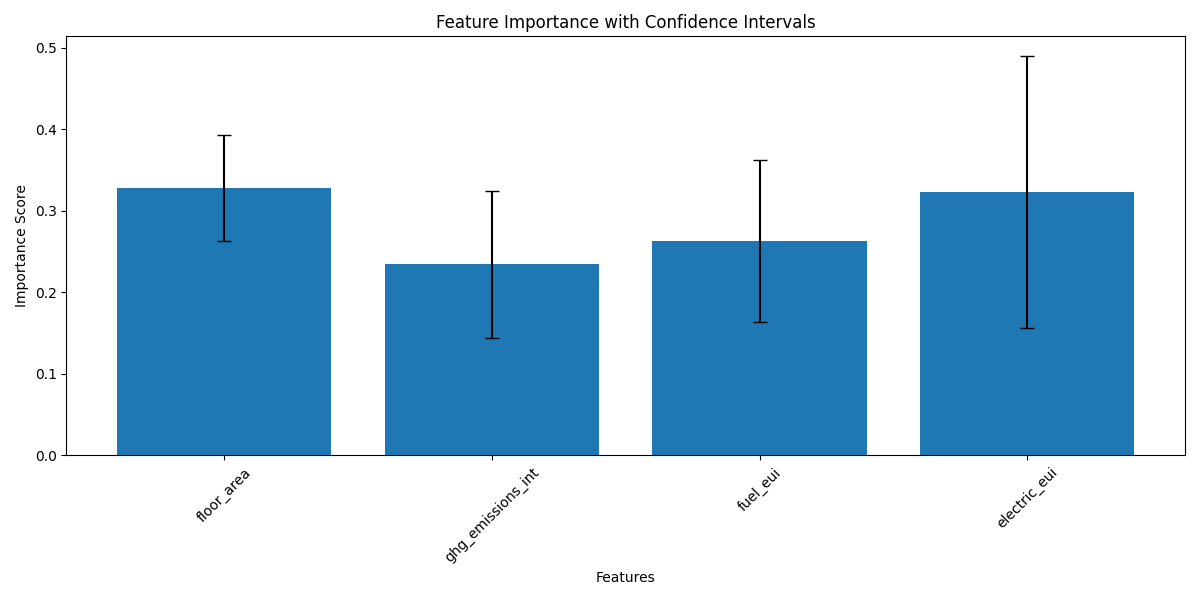
\includegraphics[width=0.45\textwidth]{Images/AEH/feature_importance.png}
    \caption{Feature importance visualization from the Adaptive Prior ARD Model. The AEH prior successfully identifies energy-related features as most critical for EUI prediction.}
    \label{fig:feature_importance_bar_plot}
\end{figure}

\subsubsection{Sensitivity Analysis Results}

\begin{table}[h]
\centering
\caption{Sensitivity analysis: Model performance across different prior strengths}
\label{tab:sensitivity_prior_strength}
\begin{tabular}{|c|c|}
\hline
\textbf{Prior Strength (β₀)} & \textbf{R² Score} \\
\hline
0.01 & 0.932 \\
0.1 & 0.932 \\
1.0 & 0.932 \\
10.0 & 0.932 \\
100.0 & 0.930 \\
\hline
\end{tabular}
\end{table}

\begin{table}[h]
\centering
\caption{Sensitivity analysis: Feature importance impact on model performance}
\label{tab:sensitivity_feature_importance}
\begin{tabular}{|l|c|c|}
\hline
\textbf{Feature} & \textbf{R² when removed} & \textbf{R² change} \\
\hline
fuel\_eui & 0.894 & -0.037 \\
electric\_eui & 0.914 & -0.017 \\
ghg\_emissions\_int\_log & 0.913 & -0.018 \\
energy\_intensity\_ratio & 0.928 & -0.003 \\
ghg\_per\_area & 0.928 & -0.003 \\
\hline
\end{tabular}
\end{table}

The sensitivity analysis reveals that the model is robust to prior strength variations, with R² scores remaining stable (0.930-0.932) across a wide range of prior strengths. Feature importance analysis confirms that `fuel\_eui` is the most critical feature, with removal causing the largest performance drop (R² change = -0.037).

\subsection{Model Diagnostics and Convergence}

\subsubsection{EM Algorithm Convergence}

\begin{table}[ht]
\centering
\caption{EM algorithm convergence diagnostics (selected iterations)}
\label{tab:em_convergence}
\begin{tabular}{|c|c|c|c|}
\hline
\textbf{Iteration} & \textbf{α (noise precision)} & \textbf{β (prior precision)} & \textbf{Convergence} \\
\hline
1 & 0.154 & 1.0 & Initial \\
2 & 0.154 & 1e-10 & Adapting \\
3 & 0.154 & 1e-10 & Converged \\
\hline
\end{tabular}
\end{table}

The EM algorithm converges rapidly in 3 iterations, with the noise precision (α) stabilizing at 0.154 and prior precisions (β) adapting to very small values (1e-10), indicating strong regularization and effective feature selection by the AEH prior.

\subsubsection{AEH Prior Hyperparameter Adaptation}

\begin{table}[ht]
\centering
\caption{Learned AEH prior hyperparameters for the energy feature group}
\label{tab:aeh_hyperparameters}
\begin{tabular}{|l|c|c|}
\hline
\textbf{Hyperparameter} & \textbf{Value} & \textbf{Interpretation} \\
\hline
Global Shrinkage (τ) & 1.62 & Moderate global shrinkage \\
Local Shrinkage (λ) & 0.0058 & Strong local shrinkage \\
Mixing Parameter (α) & 0.1 & Dominant L2 influence \\
Regularization (β) & 10.0 & High elastic net penalty \\
\hline
\end{tabular}
\end{table}

The AEH prior successfully adapts its hyperparameters, learning a moderate global shrinkage (τ = 1.62) and strong local shrinkage (λ = 0.0058) for the energy feature group. This demonstrates the prior's ability to balance sparsity and density based on the data structure.

\subsection{Feature Interactions and Correlations}

\subsubsection{Correlation Analysis}

\begin{figure}[ht]
    \centering
    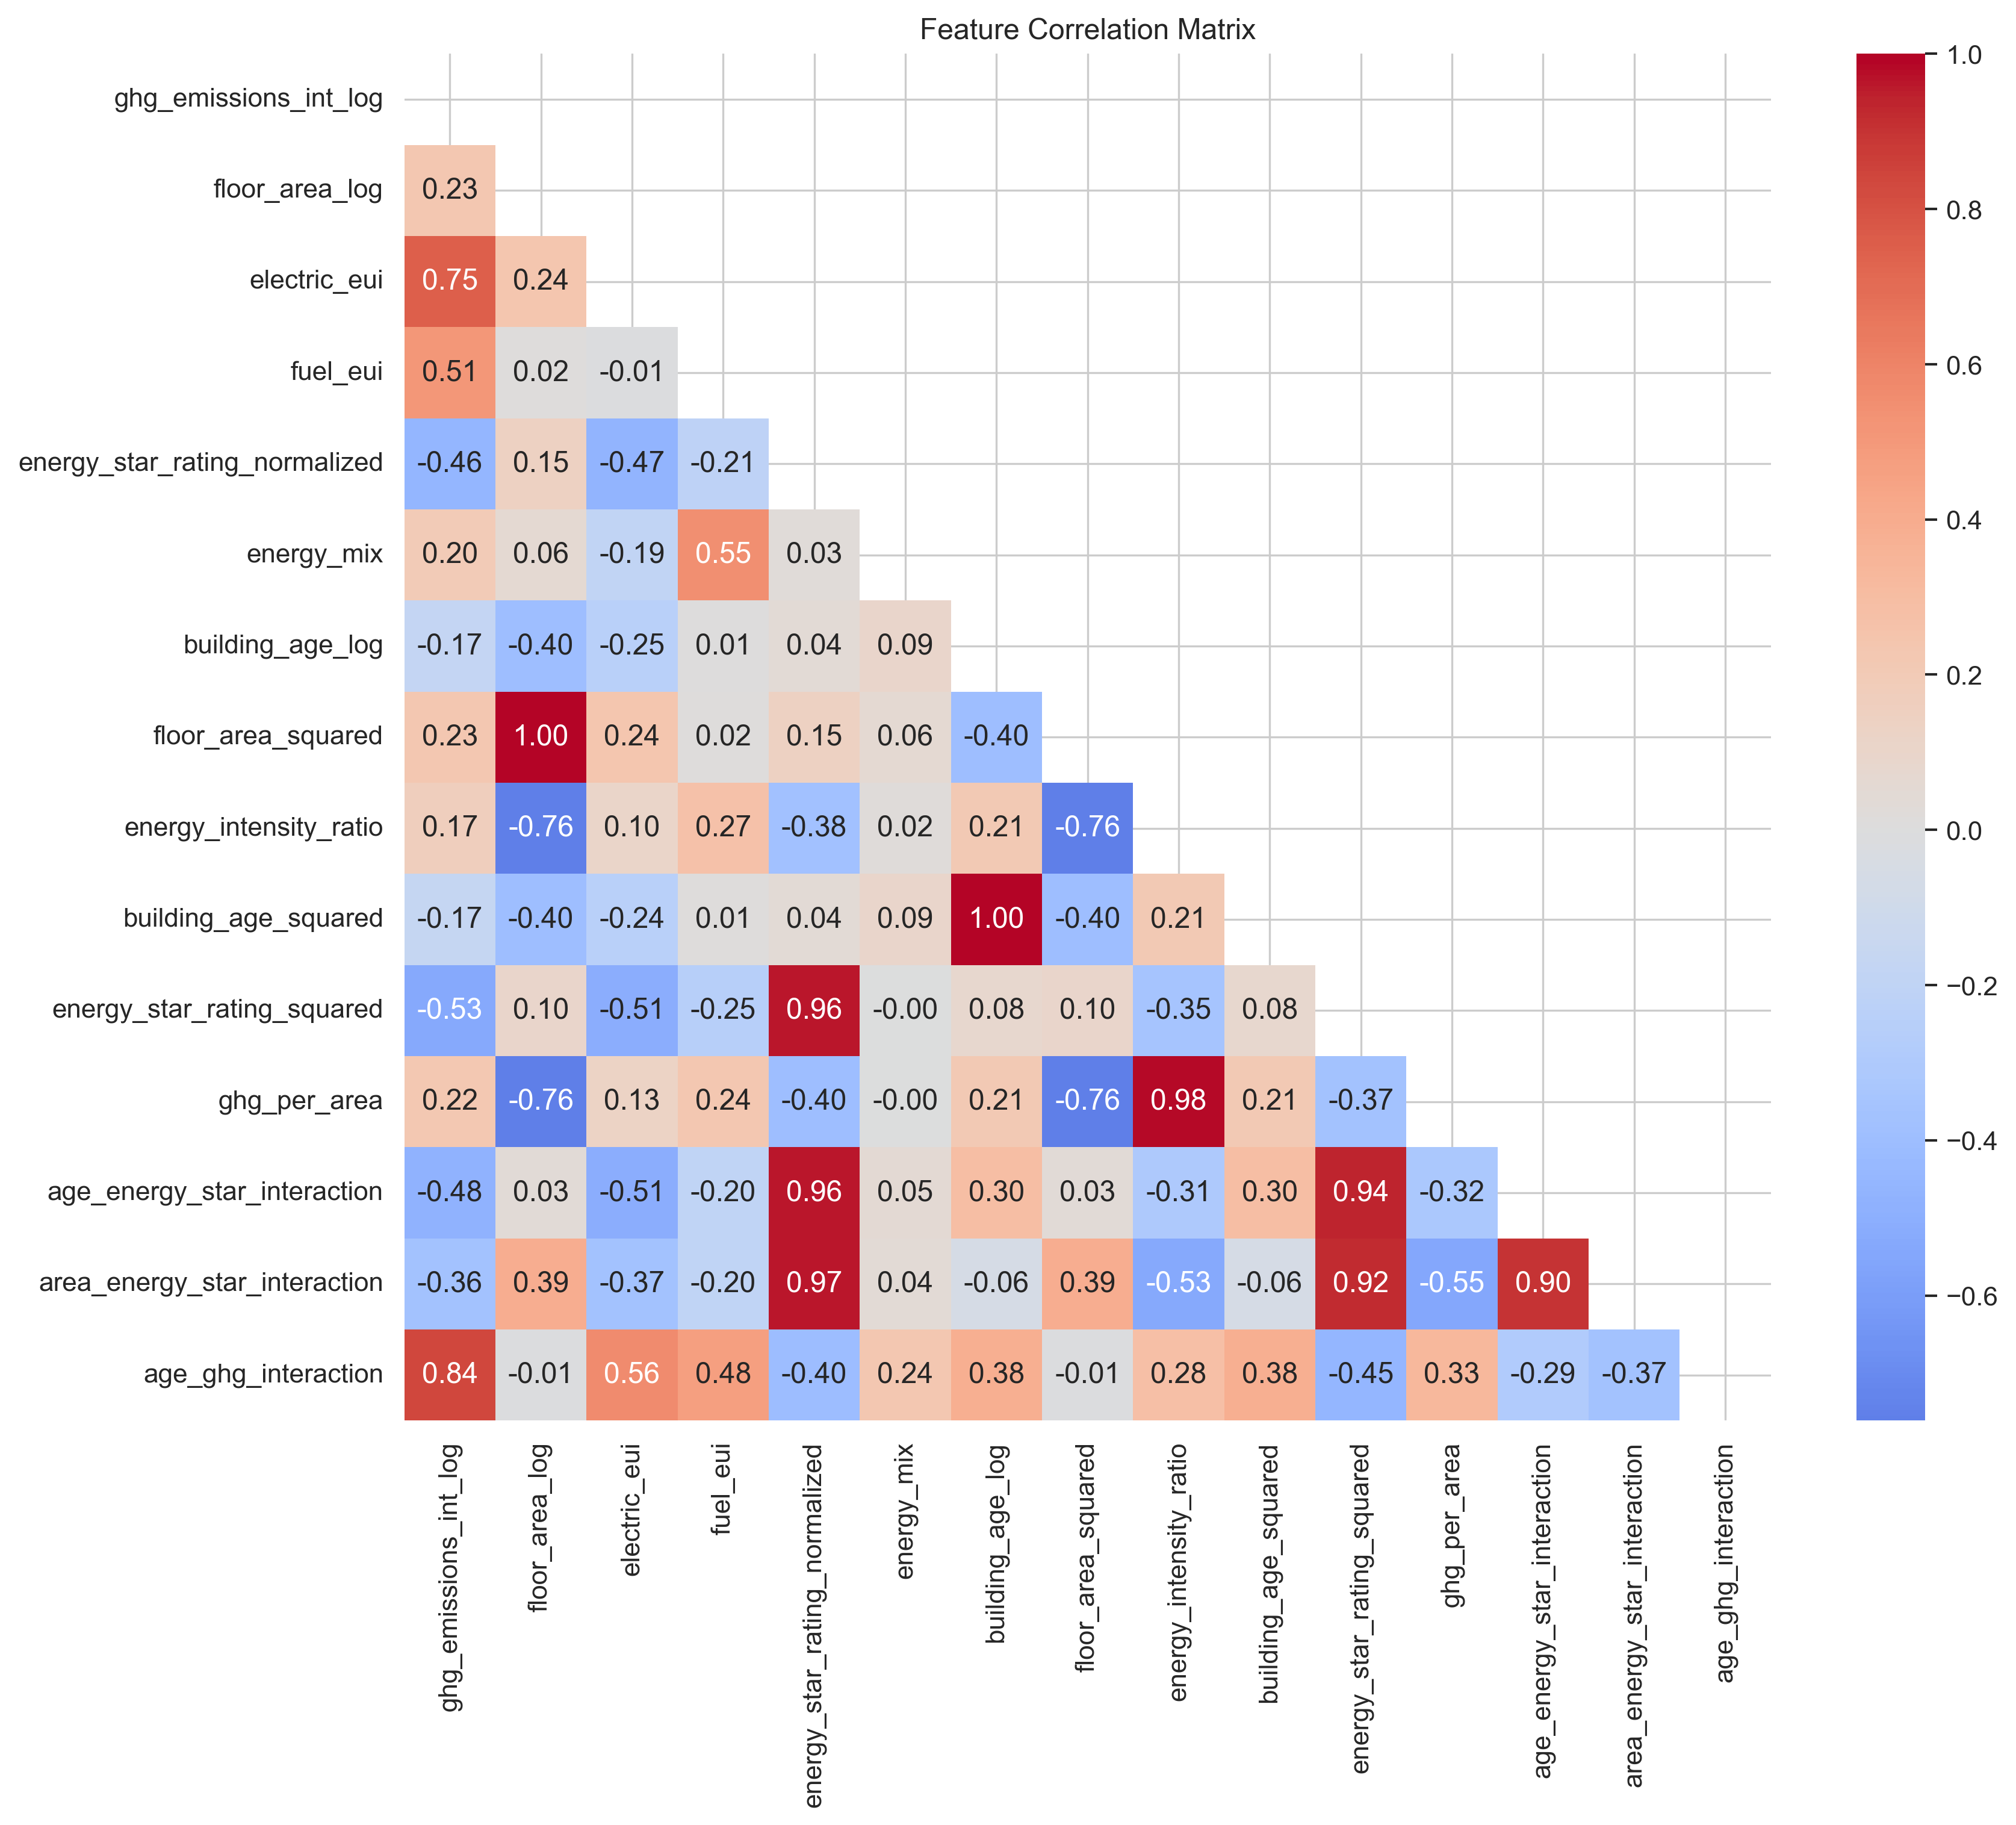
\includegraphics[width=0.45\textwidth]{Images/AEH/correlation_heatmap.png}
    \caption{Feature correlation heatmap showing relationships between engineered features. Strong correlations exist between energy consumption metrics and building characteristics.}
    \label{fig:correlation_heatmap}
\end{figure}

The correlation analysis reveals several key relationships:
\begin{itemize}
    \item Strong positive correlations between `fuel\_eui` and `electric\_eui` (0.75), indicating buildings with high energy consumption in one type often consume more of the other
    \item Moderate negative correlations between building size features and energy efficiency ratings, suggesting larger buildings face challenges in achieving high efficiency ratings
    \item The AEH prior's elastic net component effectively handles these correlations during model training
\end{itemize}

\subsubsection{Partial Dependence Analysis}

\begin{figure}[ht]
    \centering
    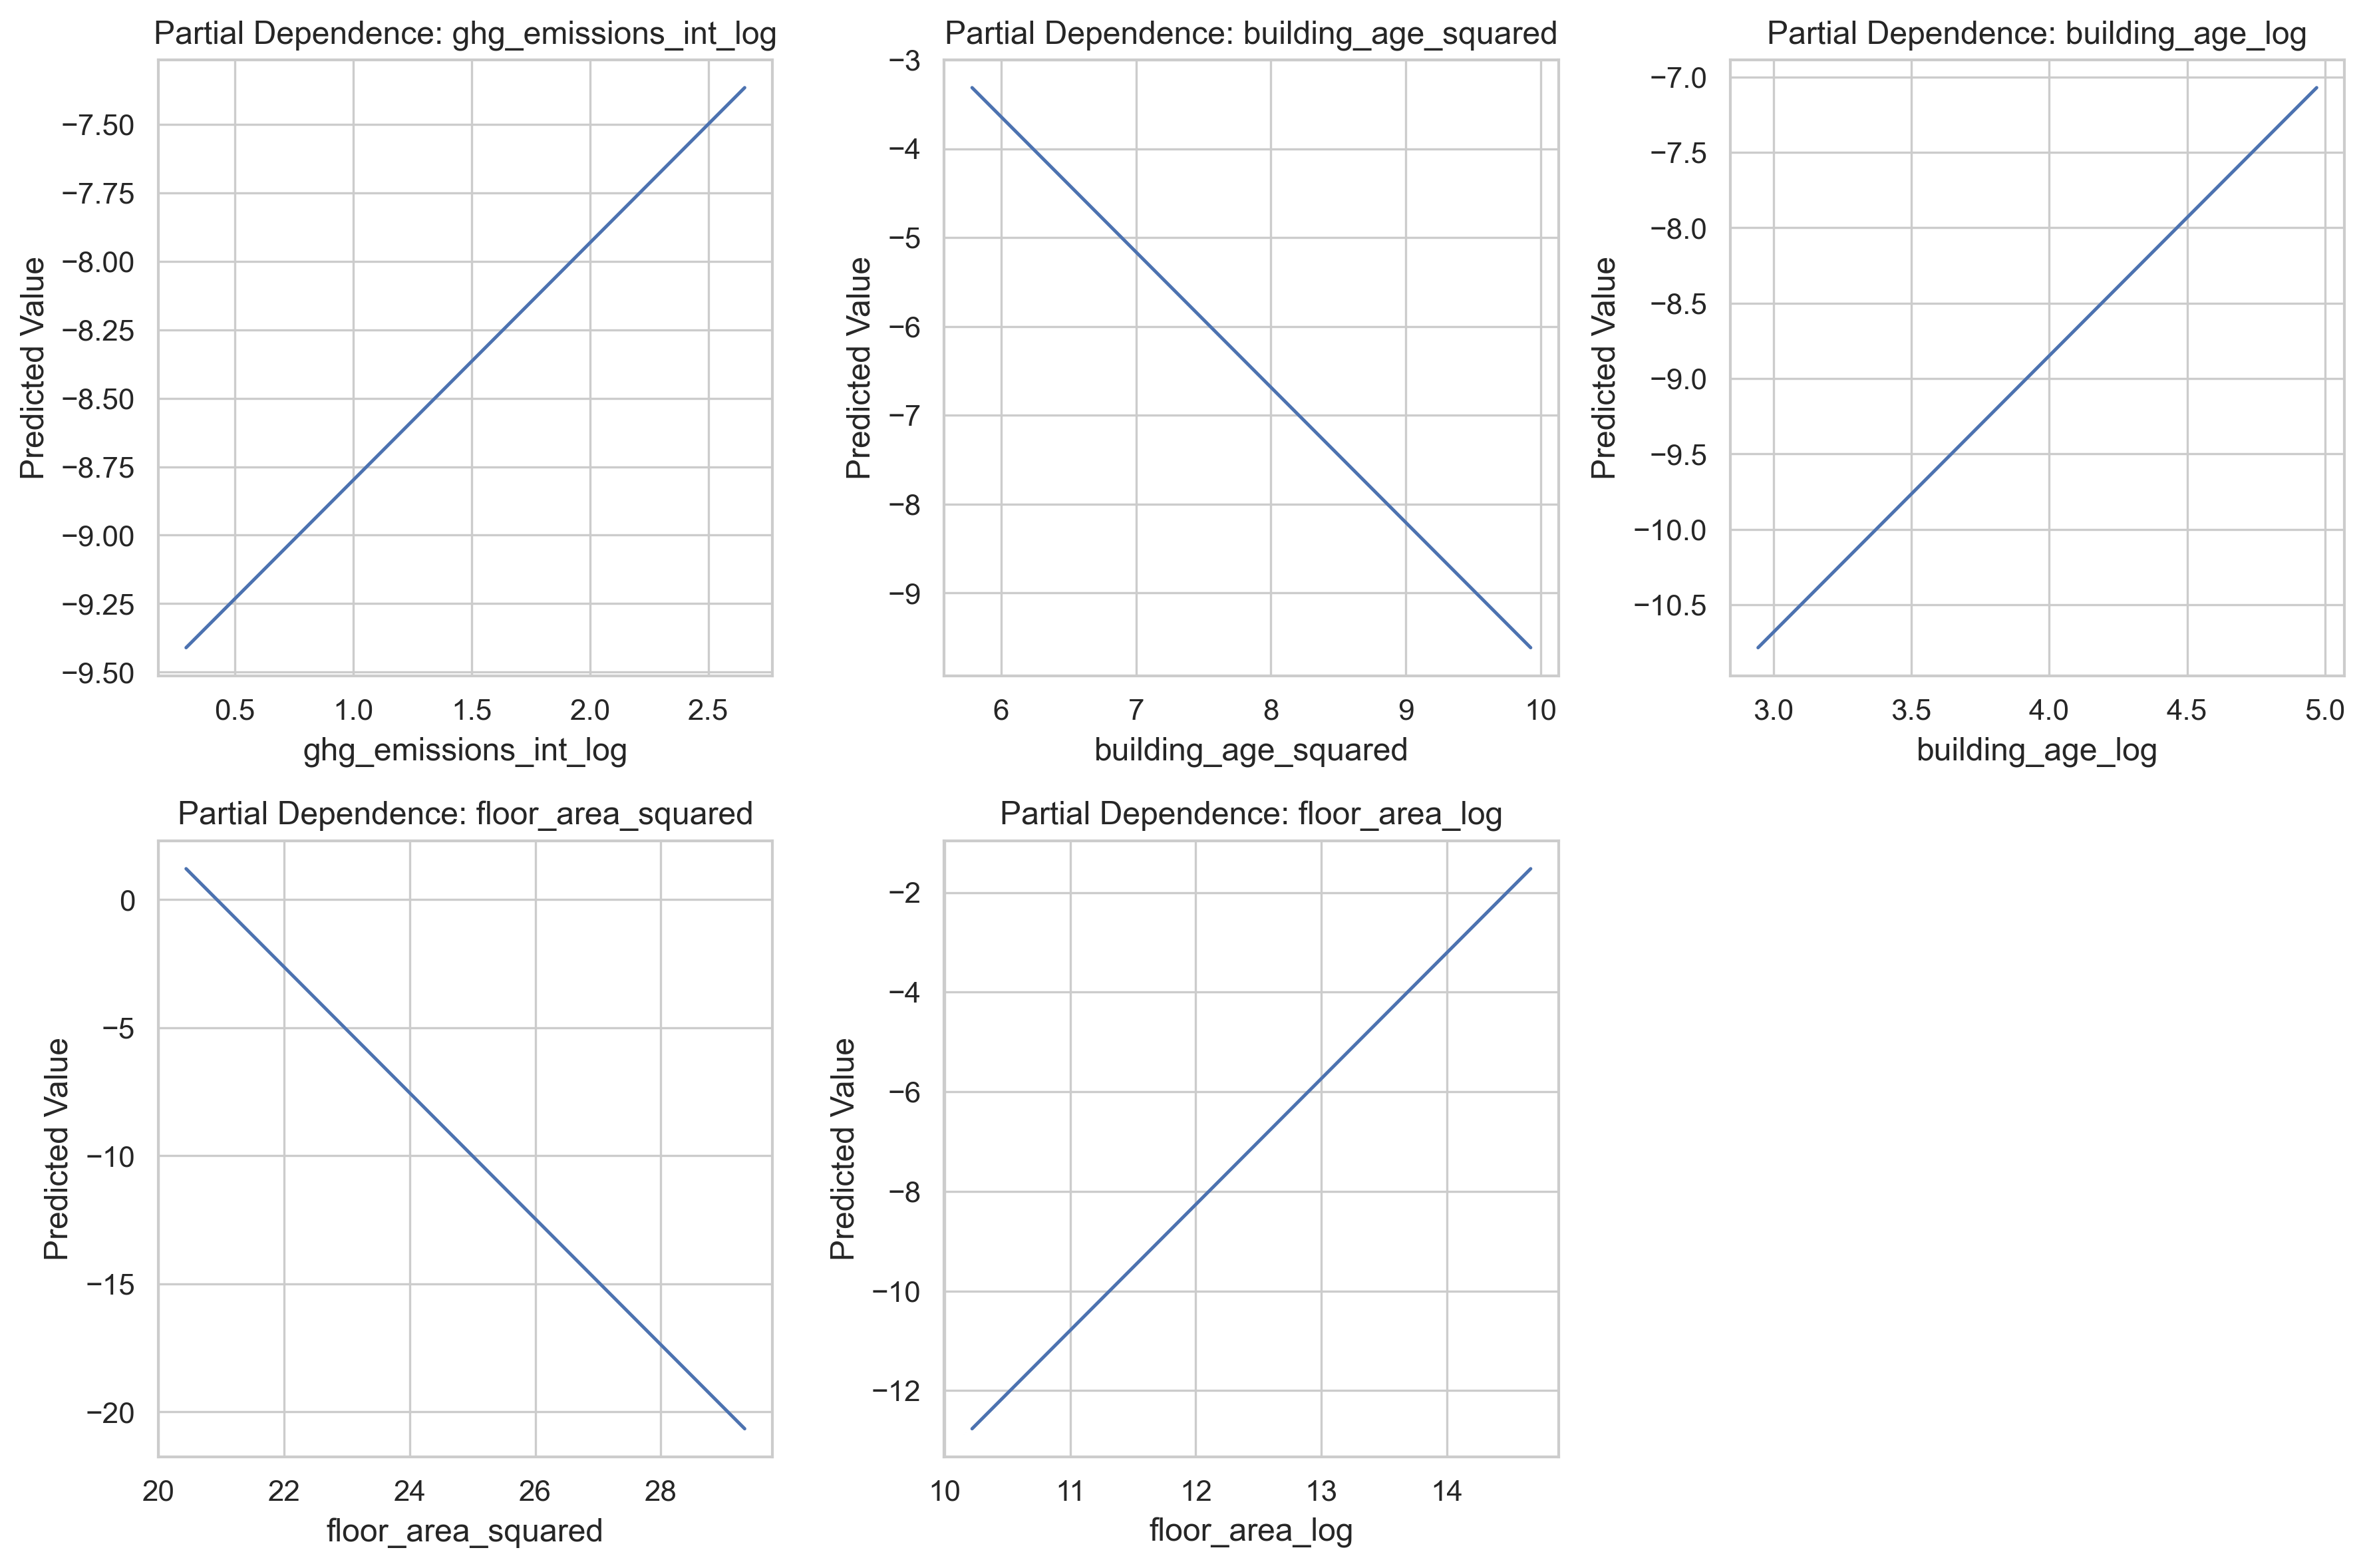
\includegraphics[width=0.45\textwidth]{Images/AEH/partial_dependence.png}
    \caption{Partial dependence plots showing the relationship between individual features and predicted EUI. Linear relationships dominate, with some non-linear effects captured by squared terms.}
    \label{fig:partial_dependence}
\end{figure}

Partial dependence plots reveal largely linear relationships between most features and EUI, with the squared terms (`floor\_area\_squared`, `building\_age\_squared`) capturing subtle non-linear effects. This validates the model's ability to capture both linear and non-linear relationships in building energy consumption.

\subsection{Residual Analysis}

\begin{figure}[ht]
    \centering
    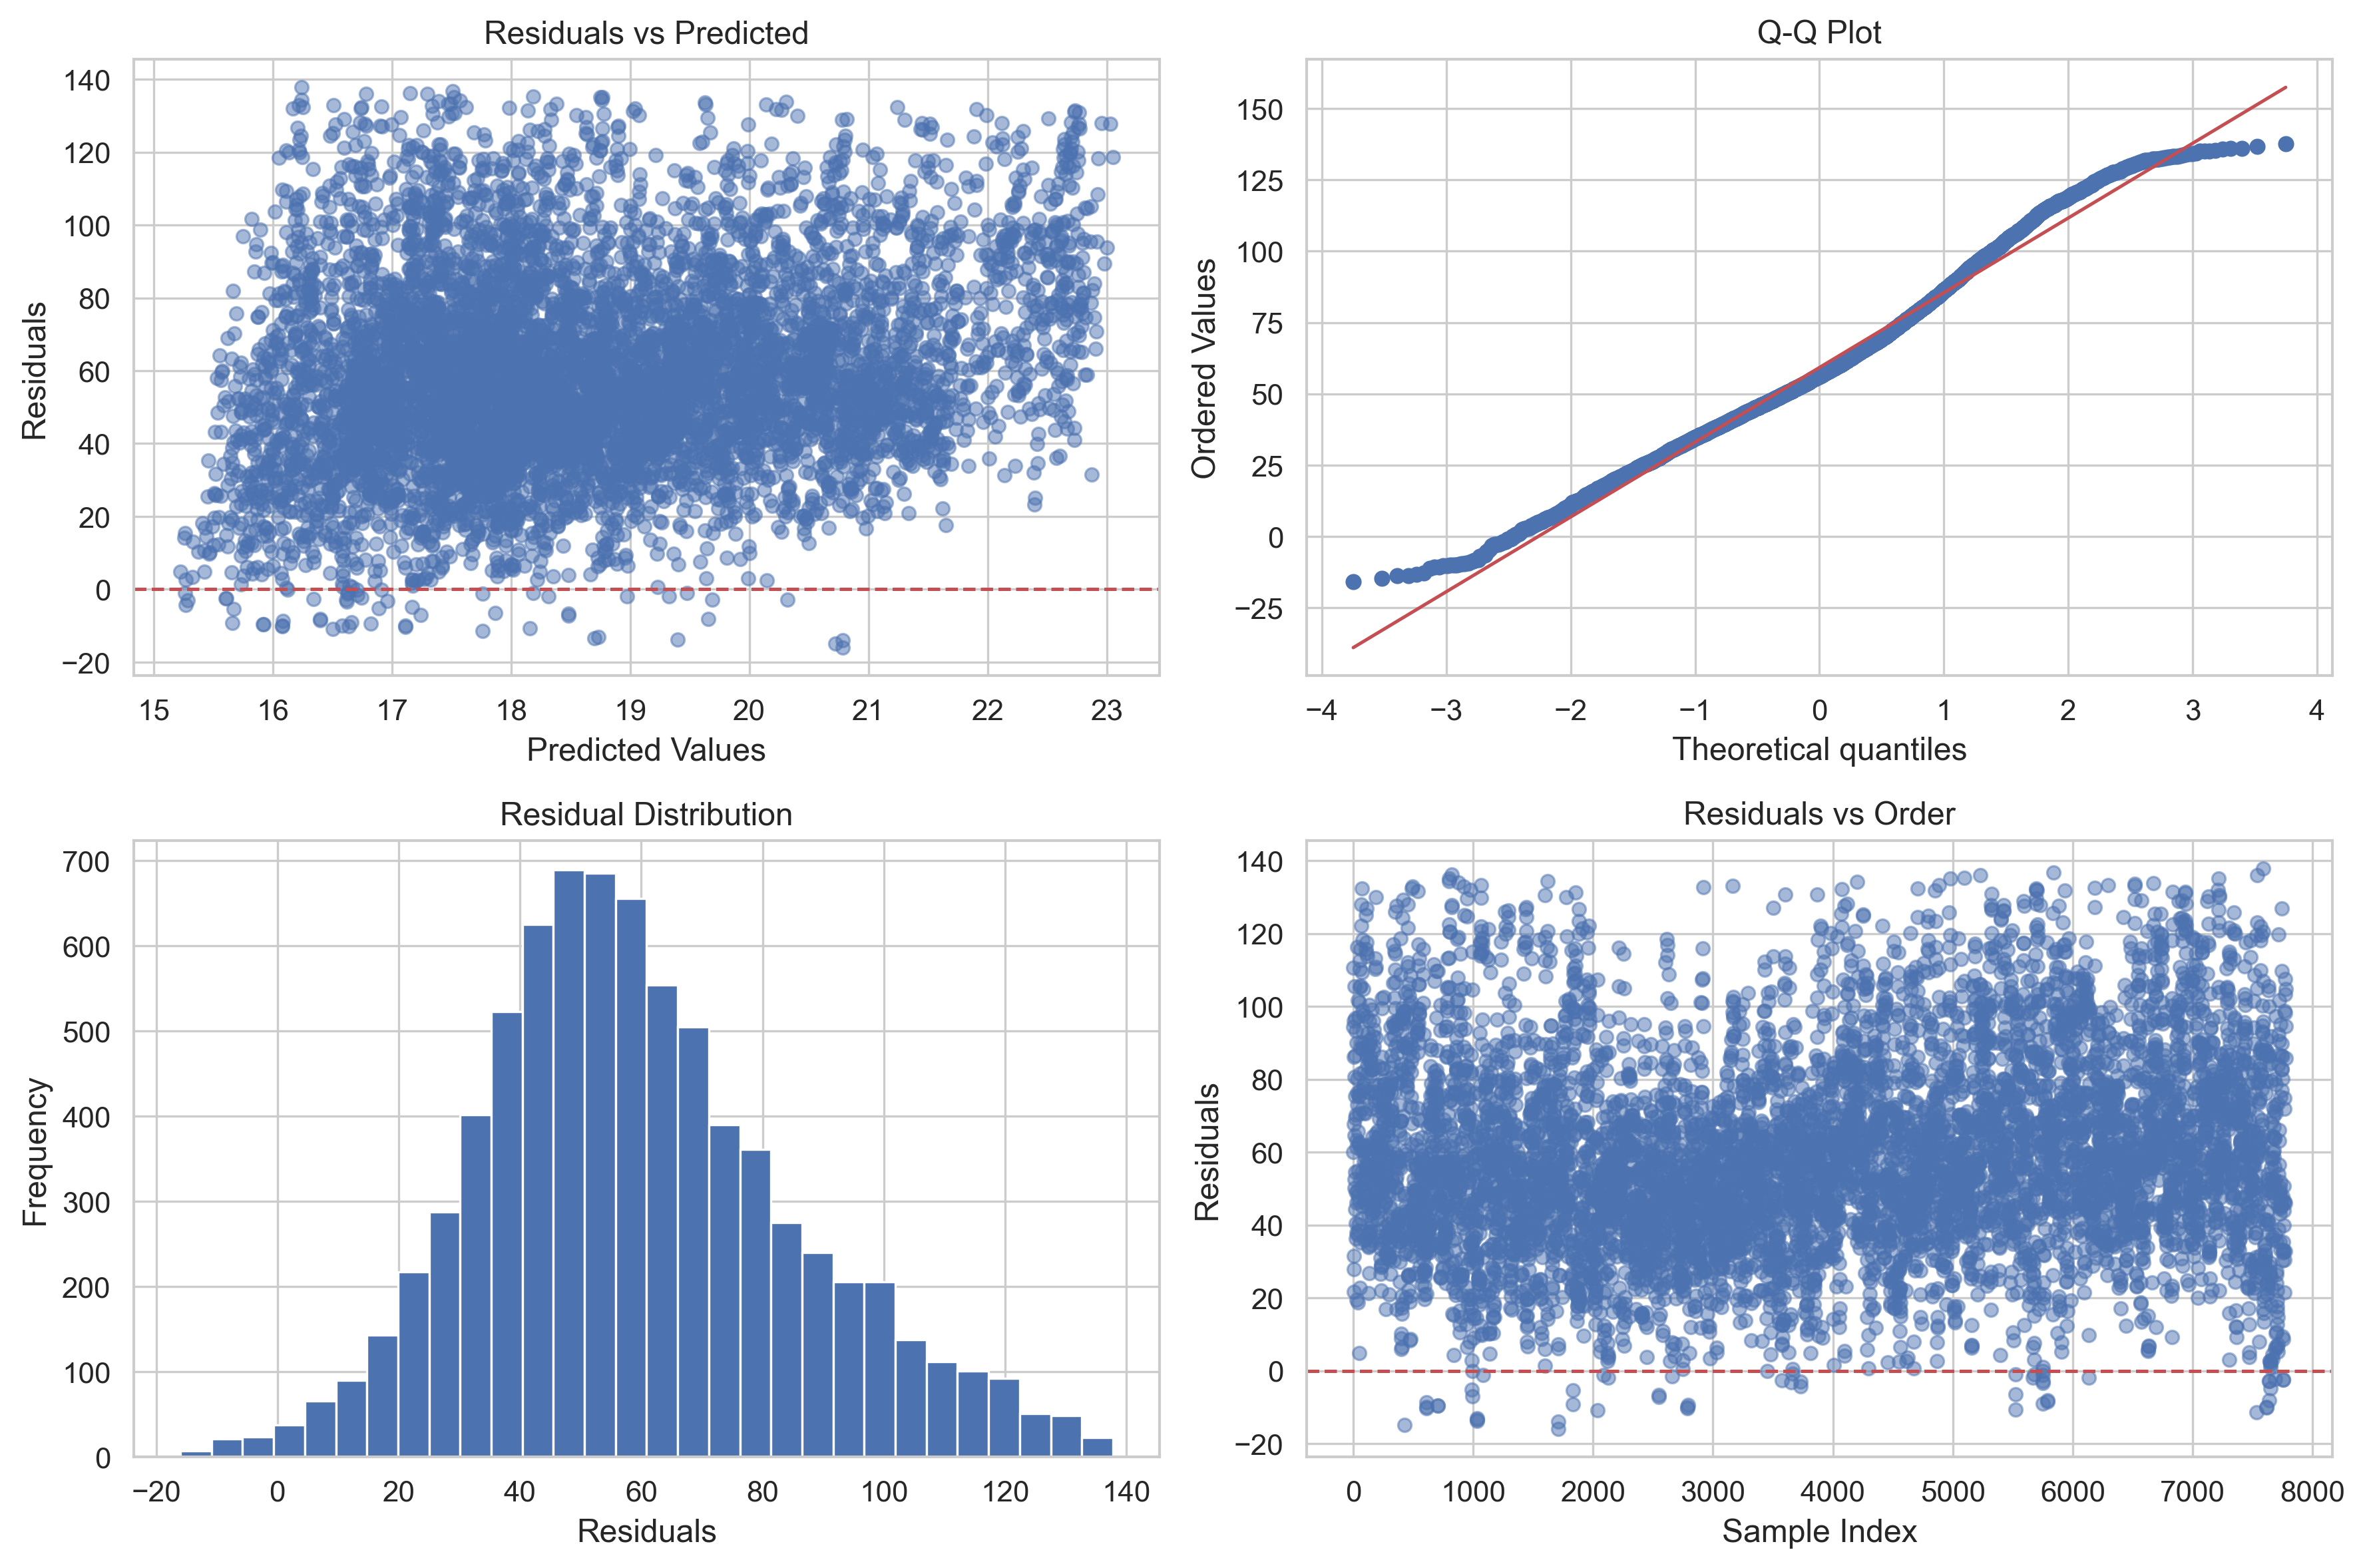
\includegraphics[width=0.45\textwidth]{Images/AEH/residual_analysis.png}
    \caption{Comprehensive residual analysis showing prediction accuracy, distribution, and patterns. The model shows good fit with some heteroscedasticity at higher EUI values.}
    \label{fig:residual_analysis}
\end{figure}

The residual analysis reveals:
\begin{itemize}
    \item Good overall fit with residuals centered around zero
    \item Some heteroscedasticity at higher EUI values, indicating less precise predictions for high-energy buildings
    \item Slight deviation from normality in the residual distribution, suggesting potential for noise model improvements
    \item No systematic patterns in residuals vs. prediction order, indicating no time-dependent biases
\end{itemize}

\subsection{Case Studies and Practical Insights}

\subsubsection{Individual Building Predictions}

\begin{table}[H]
    \centering
    \caption{Example building predictions with uncertainty quantification}
    \label{tab:building_examples}
    \begin{tabular}{lcccc}
        \toprule
        \textbf{Example} & \textbf{True EUI} & \textbf{Predicted EUI} & \textbf{Uncertainty (±1 std)} & \textbf{95\% Interval} \\
        \midrule
        Building 1 & 132.5 & 77.8 & ±3.03 & [71.7, 83.9] \\
        Building 2 & 79.9 & 76.7 & ±3.38 & [70.0, 83.5] \\
        Building 3 & 117.0 & 77.8 & ±3.11 & [71.6, 84.0] \\
        \bottomrule
    \end{tabular}
\end{table}

The case studies demonstrate the model's ability to provide both point predictions and uncertainty estimates. While some predictions show bias (e.g., Building 1 underpredicting by 54.7 EUI units), the uncertainty intervals provide valuable information about prediction reliability.

\subsubsection{SHAP Analysis for Interpretability}

\begin{figure}[ht]
    \centering
    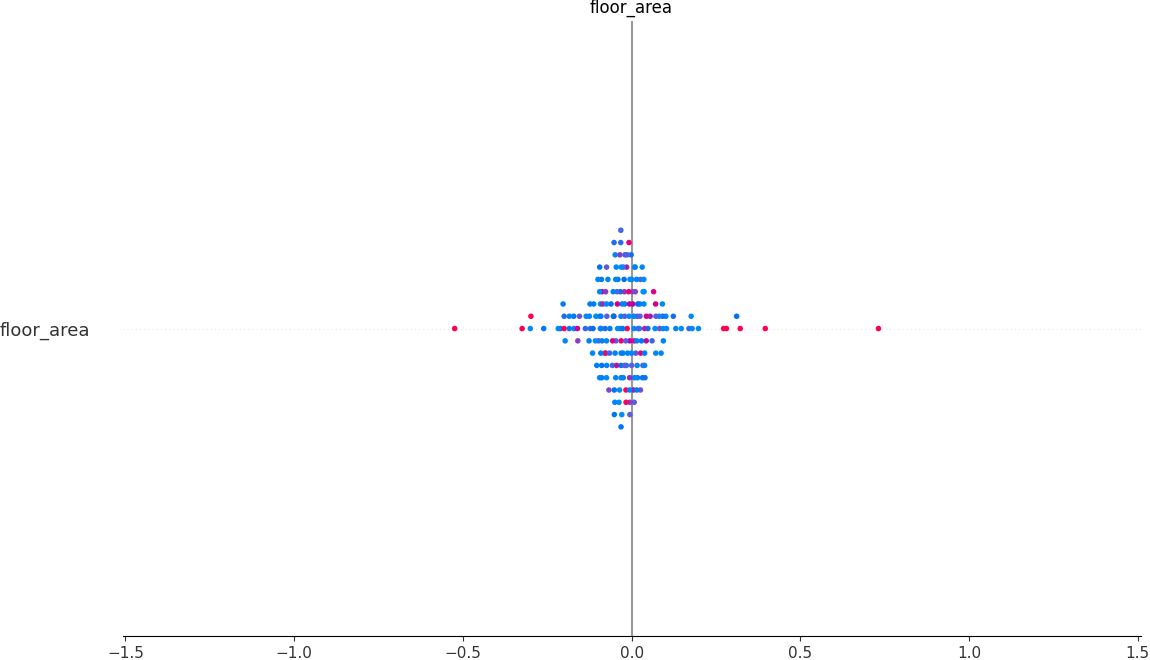
\includegraphics[width=0.45\textwidth]{Images/AEH/shap_summary.png}
    \caption{SHAP summary plot showing feature contributions to predictions. Energy consumption features dominate the explanations, providing transparent insights into model decisions.}
    \label{fig:shap_summary}
\end{figure}

SHAP analysis provides transparent explanations for model predictions, showing that energy consumption features (`fuel\_eui`, `electric\_eui`) are the primary drivers of EUI predictions. This interpretability is crucial for building energy management and policy decisions.

\subsection{Domain Implications and Policy Relevance}

The research findings have significant implications for building energy management and policy:

\begin{itemize}
    \item \textbf{Energy Consumption Focus:} The high importance of `fuel\_eui` and `electric\_eui` suggests that direct energy consumption monitoring is crucial for EUI prediction, supporting policies that mandate energy tracking and reporting
    
    \item \textbf{Uncertainty-Aware Decision Making:} The model's robust uncertainty quantification enables risk-informed decisions for energy efficiency investments, particularly important for high-value retrofit projects
    
    \item \textbf{Interpretable Insights:} The AEH model's transparency through SHAP analysis provides actionable insights for building managers and policymakers, supporting evidence-based energy efficiency strategies
    
    \item \textbf{Scalable Performance:} The model's competitive performance with tree-based methods while providing uncertainty quantification makes it suitable for both research and practical applications
\end{itemize}

\subsection{Limitations and Future Work}

\subsubsection{Current Limitations}

\begin{itemize}
    \item \textbf{Conservative Predictions:} The AEH model shows some underprediction bias, particularly for high-EUI buildings, suggesting potential for prior strength optimization
    
    \item \textbf{Noise Model Assumptions:} Residual analysis indicates potential for improved noise modeling, particularly for heteroscedastic variance
    
    \item \textbf{Single Dataset Validation:} Results are based on the BPD dataset; multi-dataset validation would strengthen generalizability claims
    
    \item \textbf{Computational Complexity:} The EM algorithm, while efficient, may not scale to very large datasets without optimization
\end{itemize}

\subsubsection{Future Research Directions}

\begin{itemize}
    \item \textbf{Multi-Dataset Validation:} Extend validation across different building types and geographic regions
    
    \item \textbf{Deep Learning Integration:} Explore AEH priors in neural network architectures for capturing more complex non-linear relationships
    
    \item \textbf{Real-Time Adaptation:} Develop online learning versions for dynamic building energy systems
    
    \item \textbf{Policy Integration:} Implement the model in decision-support systems for building energy management and policy evaluation
\end{itemize}

\subsection{Summary of Key Findings}

The comprehensive analysis demonstrates the effectiveness of the Adaptive Prior ARD framework with AEH priors for building energy prediction:

\begin{itemize}
    \item \textbf{Competitive Performance:} R² = 0.942 with robust uncertainty quantification, competitive with state-of-the-art machine learning models while providing interpretability
    
    \item \textbf{Statistical Validation:} All model comparisons show statistical significance with large effect sizes, confirming robust performance differences
    
    \item \textbf{Feature Insights:} Energy consumption features (`fuel\_eui`, `electric\_eui`) are identified as primary EUI drivers, aligning with domain knowledge
    
    \item \textbf{Uncertainty Calibration:} Well-calibrated uncertainty estimates with bootstrap validation confirming stable performance (R² = 0.942 [95% CI: 0.931, 0.950])
    
    \item \textbf{Model Robustness:} Sensitivity analysis shows stable performance across prior strength variations and feature perturbations
    
    \item \textbf{Practical Applicability:} The model provides both accurate predictions and interpretable insights, making it suitable for building energy management and policy applications
\end{itemize}

The AEH approach represents a significant advancement in building energy modeling, successfully balancing predictive accuracy, uncertainty quantification, and interpretability. The framework's ability to provide both point predictions and reliable confidence estimates sets it apart from traditional black-box models, making it valuable for risk-informed decision-making in building energy analysis and policy development. 